% !TEX root = ./report.tex

\clearpage
\section{Background}
\label{background}

\subsection{The Regionalized Value-State Dependence Graph}
\label{background:RVSDG}

The \textit{Regionalized Value State Dependence Graph}~\cite{RVSDG:HiPEACpaper}
(RVSDG) is a \textit{directed acyclic demand-based dependence graph},
consisting of nodes representing computations and edges representing the
dependencies between nodes. Each node has inputs and outputs connected through
edges. The arity and order of inputs and outputs depend on the operation the
node represents.

Figure~\ref{fig:simple_node_RVSDG_ex} exemplifies how the C/C++ code on the left
can be represented as a directed acyclic demand-based dependence graph, depicted
in the figure on the right. The nodes in the figure represent operations in a
program, while the edges between the nodes show the dependencies nodes have to
each other, and this gives the order of execution.

In all RVSDG examples depicted in this report, the order of inputs in a node
starts with the first input being the edge closest to the bottom left corner of
the node, clockwise.

\begin{centering}
	\noindent\begin{minipage}{0.36\textwidth}
		\begin{CenteredBox}
		\begin{lstlisting}[label={lst:simple_node_RVSDG_ex},
style=minipage_customcpp, basicstyle=\fontsize{14}{1}]
x = (y*2) / (z+2);
		\end{lstlisting}
		\end{CenteredBox}
	\end{minipage}
	\noindent\begin{minipage}{0.55\textwidth}
		\captionsetup{type=figure}
		\includegraphics[width=\textwidth]{figures/simple_node_RVSDG_ex}
	\end{minipage}
	\captionof{figure}{Example of an RVSDG subgraph equivalent to the C/C++
on the left.}
	\label{fig:simple_node_RVSDG_ex}
\end{centering}

\subsubsection{Edges}

The RVSDG has two types of edges: data dependence edges and state dependence
edges. They represent data and state dependencies operations have to another,
respectively. An example of data dependence edges are the operands used in an
addition, such as in Figure~\ref{fig:simple_node_RVSDG_ex}.

State dependence edges are used to preserve the semantics of the program when
the program has side-effecting operations. If there are no data dependencies
between operations, giving an order to the execution of the connected
operations.

\subsubsection{Nodes}

The RVSDG has two kinds of nodes: simple nodes and complex nodes. Simple nodes
are used to represent primitive operations, such as addition and substraction.
The arity and order of inputs and outputs of any RVSDG node need to match the
operation. Figure~\ref{fig:simple_node_RVSDG_ex} is an example of an RVSDG
containing only simple nodes.

This report puts special focus on the \applyNode . An \applyNode~represents the
call site of a function. The first input argument of an \applyNode~is a link to
the function the \applyNode~invokes. The rest of the inputs of an
\applyNode~need to match the order and arity of the input arguments of the
function-node it's linked to. Likewise, the results also need to match the same
order and arity as the outputs of the function-node.

Complex nodes contain an RVSDG subgraph, which is why they are also referred to
as \textit{regions}. Differing from the simple nodes with their contained
subgraph, complex nodes normally ``gate'' the external inputs they get from the
rest of the RVSDG through to internal outputs. Consequently, they also have
internal inputs which can gate through to their external outputs, connecting the
dependencies to the rest of the RVSDG. An example of this is depicted in
Figure~\ref{fig:complex_node_mapping_ex}.

\begin{figure}[H]
	\centering
	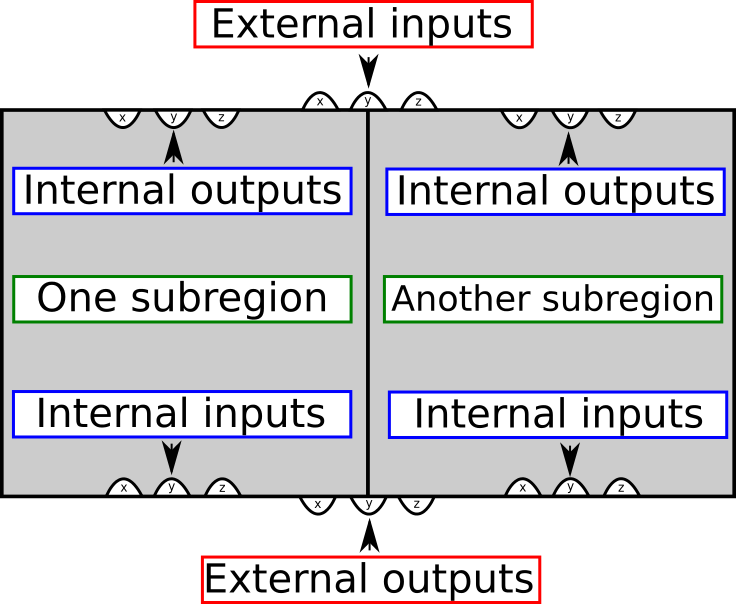
\includegraphics[width=0.7\textwidth]{figures/complex_node_mapping_ex}
	\caption{A minimal example of a complex node, showing which inputs/outputs
are external/internal, and how they can have multiple subregions.}
	\label{fig:complex_node_mapping_ex}
\end{figure}

Figure~\ref{fig:fib_phi} illustrates how complex nodes can contain both simple-
and complex- nodes, and how complex nodes have internal and external outputs.

The complex nodes of an RVSDG relevant for this report are as follows:

\begin{itemize}

\item \textbf{$\gamma$-nodes: N-way statements}

\textit{$\gamma$-nodes} represent conditional statements. Each $\gamma$-node has
a predicate as first input. All other edges passing as inputs to the
$\gamma$-node are edges its subregions depend upon. All subregions must have the
same order and arity of internal inputs and outputs, even if the subgraph in
each region does not depend on all of the internal outputs.

A $\gamma$-node is equivalent to a \textit{switch-case} without fall-through in
C/C++. Each case of the switch statement corresponds to a subregion of the
$\gamma$-node. Hence, a simple \textit{if-statement} with no else-clause can be
represented by a $\gamma$-node with two subregions. The true subregion contains
the RVSDG subgraph that represents the body of the if-statement, whereas the
false subregion of the $\gamma$-node simply routes all inputs through. See
Figure~\ref{fig:simple_if} for an example of a $\gamma$-node.

\begin{centering}
	\noindent\begin{minipage}{0.36\textwidth}
		\begin{CenteredBox}
		\begin{lstlisting}[label={lst:simple_if}, style=minipage_customcpp,
basicstyle=\fontsize{14}{1}]
if((z-2) != 0 ){
	x = (y*2) / (z+2);
}
		\end{lstlisting}
		\end{CenteredBox}
	\end{minipage}
	\noindent\begin{minipage}{0.55\textwidth}
		\captionsetup{type=figure}
		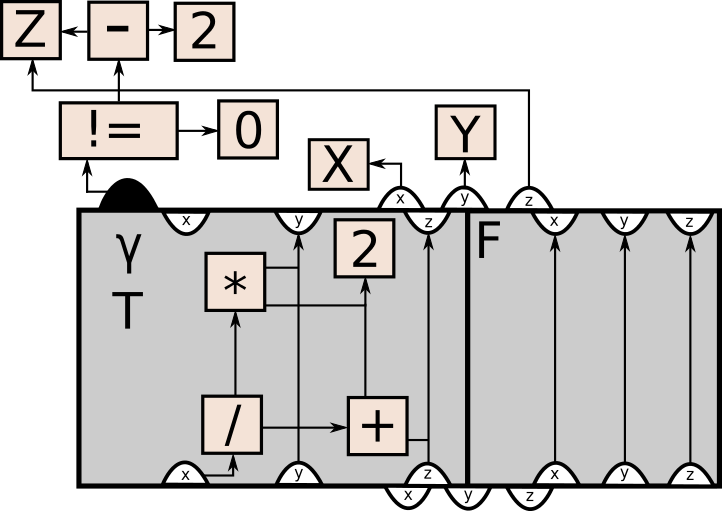
\includegraphics[width=\textwidth]{figures/simple_if_example}
	\end{minipage}
	\captionof{figure}{Example of an RVSDG subgraph on the right, depicting a
$\gamma$-node equivalent to the C/C++ if-statement on the left.}
	\label{fig:simple_if}
\end{centering}

\item \textbf{$\theta$-nodes: Tail-controlled loops}

\textit{$\theta$-nodes} represent tail controlled loops. As with
$\gamma$-nodes, its inputs (and outputs) are all the dependencies needed for the
RVSDG subgraph in its subregion.

Inside the $\theta$-node there is an extra first internal input, which is the
predicate of the tail controlled loop. If this predicate evaluates to true, the
rest of the internal inputs of the $\theta$-node are mapped to their
corresponding internal outputs. This enables the iterative behaviour of an RVSDG
$\theta$-node. However, the first time the operations of the node are executed,
the external inputs are mapped to the internal outputs. Thus, the operations
represented by its contained RVSDG subgraph can be executed as a tail-controlled
loop.

A $\theta$-node is equivalent to a \textit{do-while} loop in C/C++, as shown in
Figure~\ref{fig:factorial_loop_ex}. See Listing~\ref{lst:factorial_loop_ex} for
the C/C++ code corresponding to the RVSDG depicted in
Figure~\ref{fig:factorial_loop_ex}.

\begin{centering}
	\noindent\begin{minipage}{0.36\textwidth}
		\begin{CenteredBox}
		\begin{lstlisting}[style=global_customcpp,
label={lst:fig:factorial_loop_ex}, basicstyle=\fontsize{14}{1}]
unsigned int i = 0;
unsigned long long r = 1;
do{
	i += 1;
	r *= i;
} while(i < n);
		\end{lstlisting}
		\end{CenteredBox}
	\end{minipage}
	\noindent\begin{minipage}{0.55\textwidth}
		\captionsetup{type=figure}
		\includegraphics[width=\textwidth]{figures/iterative_factorial_ex}
	\end{minipage}
	\captionof{figure}{An RVSDG subgraph on the right, depicting a
$\theta$-node equivalent to the C/C++ do-while loop on the left.}
	\label{fig:factorial_loop_ex}
\end{centering}

Other loops than tail-controlled loops can be represented by combining complex
nodes. A \textit{for-loop} can be represented by putting a $\theta$-node inside
of the \textit{true} clause of a $\gamma$-node conaining no subgraph in the
subregion representing the \textit{false} clause. This will equate to a
\textit{for-loop} if the $\gamma$-node and $\theta$-node have the same predicate
expression.

\item \textbf{$\lambda$-nodes: Functions}

\textit{$\lambda$-nodes} represent functions. They contain an RVSDG subgraph
representing the body of a function. $\lambda$-nodes only have internal
inputs, representing the dependencies given from its contained RVSDG.
Respectively, its internal outputs give the dependencies needed by the contained
RVSDG. However, its external output is what give the \applyNode s their first
link, enabling them to invoke the function represented by the
\textit{$\lambda$-node}.

When the invokation of a \textit{$\lambda$-node} is linked with an \applyNode ,
the external inputs of the \applyNode~are mapped to the internal outputs of the
\textit{$\lambda$-node}, and likewise with the external outputs and internal
inputs, respectively. This enables the evaluation of the body of the
\textit{$\lambda$-node}.

The arity and order of its internal inputs and outputs must match the arity and
order of the external inputs and outputs of all correspondingly linked
\applyNode s. Thus, the results of computations represented in the body the
\textit{$\lambda$-node} are mapped to the results of the \applyNode .

Figure~\ref{fig:factorial_loop_ex} shows an RVSDG representation of an iterative
factorial function, with its corresponding C/C++ equicalent code in
Listing~\ref{lst:factorial_loop_ex}. Figure~\ref{fig:fib_phi} and
Listings~\ref{lst:fib_phi} also illustrate the workings of $\lambda$-nodes
through the representation of an RVSDG and the equivalent C/C++ code for a
recursive fibonacci function.

\begin{centering}
	\noindent\begin{minipage}{0.37\textwidth}
		\begin{CenteredBox}
		\begin{lstlisting}[label={lst:iterative_factorial_func_ex},
style=minipage_customcpp]
unsigned long long
fac(unsigned int n){
	unsigned int i = 0;
	unsigned long long r = 1;
	do{
		i += 1;
		r *= i;
	} while(i < n);
	return r;
}
		\end{lstlisting}
		\end{CenteredBox}
	\end{minipage}
	\noindent\begin{minipage}{0.55\textwidth}
		\captionsetup{type=figure}
		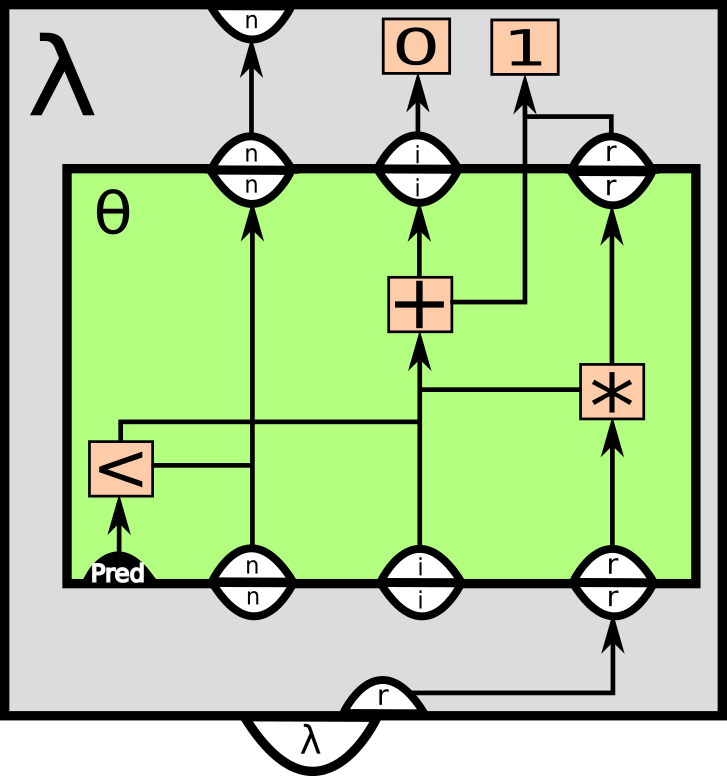
\includegraphics[width=\textwidth]{figures/iterative_factorial_func_ex}
	\end{minipage}
	\captionof{figure}{Example of an RVSDG subgraph on the right, depicting a
$\lambda$-node equivalent to the C/C++ function on the left.}
	\label{fig:iterative_factorial_func_ex}
\end{centering}

\item \textbf{$\phi$-regions: Recursive environments}

\textit{$\phi$-regions} represent recursive environments. They contain at least
one recursive \textit{$\lambda$-node}. Like the \textit{$\lambda$-node}, they
have no external inputs. However, the internal outputs of the
\textit{$\phi$-region} represent the links utilized by the \applyNode s
contained within to connect with the respective $\lambda$-nodes also
contained within the same \textit{$\phi$-region}.

The internal inputs of a \textit{$\phi$-region} \info{Nico crossed out ``receive
the function invocation links'', but what he wrote above is illegible. Ask Nico
for clarification.}receive the function invocation links from the
$\lambda$-nodes contained within. The internal inputs map to the external
outputs, thus enabling \applyNode s outside of the recursive environment to link
with the $\lambda$-nodes contained within.


An RVSDG representing the recursive fibonacci function written in C/C++ in
Listing~\ref{lst:fib_phi}, illustrates the usage of a \textit{$\phi$-region} in
Figure~\ref{fig:fib_phi}.


\begin{centering}
	\noindent\begin{minipage}{0.37\textwidth}
		\begin{CenteredBox}
		\begin{lstlisting}[label={lst:recursive_factorial_func_ex},
style=minipage_customcpp]
unsigned long long
fac(unsigned int n){
	if(n > 1){
		return n*fac(n-1)
	}
	return n;
}
		\end{lstlisting}
		\end{CenteredBox}
	\end{minipage}
	\noindent\begin{minipage}{0.55\textwidth}
		\captionsetup{type=figure}
		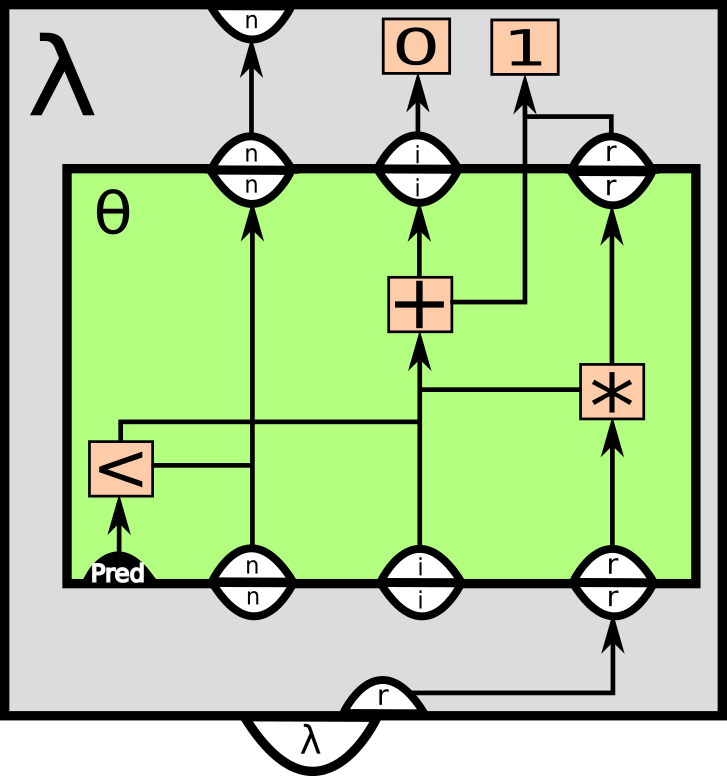
\includegraphics[width=\textwidth]{figures/iterative_factorial_func_ex}
	\end{minipage}
	\captionof{figure}{Example of an RVSDG subgraph on the right, depicting a
$\phi$-region equivalent to the recursive C/C++function on the left.}
	\label{fig:recursive_factorial_func_ex}
\end{centering}

\end{itemize}
